%!TEX encoding = UTF-8 Unicode
%!TEX root = ../easy-bindings.tex


\chapter{Tutorial}

\section{Introduction}

À partir de mac OS X 10.3 (Panther), le pattern MVC\index{MVC} (\emph{Model View Controller}) peut être mis en œuvre au moyen des \emph{Cocoa Bindings}. Ceux-ci ont perduré jusqu'aux systèmes actuels, et notamment peuvent actuellement être exprimés en Swift.

La technique préconisée par Apple pour exprimer le pattern MVC est d'écrire les \emph{bindings} directement dans l'interface graphique \emph{Interface Builder} de \emph{Xcode}. Cette approche, si elle est simple pour des petits programmes d'exemple, présente à notre avis plusieurs inconvénients pour des projets importants :
\begin{itemize}
  \item à la moindre erreur, le \emph{binding} ne fonctionne pas, ou assez souvent il en résulte un \emph{crash} de l'application ;
  \item suite à un changement de nom d'une propriété, il faut revoir tous les \emph{outlets} qui lui sont liés, en balayant les multiples items graphiques ;
  \item les valeurs transmises sont des objets Objective-C : les entiers, structures, énumérations sont convertis en instances de \texttt{NSNumber} ou de \texttt{NSValue}, les objets en instance de \texttt{NSObject}, perdant ainsi toute possibilité de vérification statique de la correction des types. 
\end{itemize}

Si tous ces points ne sont pas gênants pour un petit exemple, il s'avère en pratique que la maintenance d'une application comportant de nombreux \emph{bindings} est plus compliquée qu'il n'y paraît. Comme il n'y a pas de possibilité de vérification statique à la compilation, au moindre changement on doit s'astreindre à passer en revue dans \emph{Interface Builder} tous les \emph{outlets} : en pratique, il est fatal d'en oublier. L'erreur peut apparaître bien longtemps après la modification, si la fonction concernée n'est que peu utilisée.


\tpp{eb} est un outil facilitant la mise en œuvre du pattern MVC\index{MVC} (\emph{Model View Controller}) pour des applications Mac OS X écrites en Swift :
\begin{itemize}
  \item \emph{Interface Builder} est utilisé uniquement pour dessiner l'interface, et définir les \emph{outlets} ;
  \item aucune information de \emph{binding} n'apparaît dans \emph{Interface Builder} ;
  \item un texte \emph{Easy Bindings} est écrit pour définir les modèles et les bindings ;
  \item la compilation par l'outil \tpp{eb} de ce texte engendre du code \emph{Swift} prêt à être compilé.
\end{itemize}

Cet outil en fait va plus loin que la seule définition des \emph{bindings} :
\begin{itemize}
 \item il permet la définition des préférences ;
 \item il permet la définition des documents, y compris sauvegarde sur fichier et leur lecture ;
 \item le code engendré permet une vérification statique de la correction des bindings ;
 \item il engendre du code code qui à l'exécution maintient une liste des objets alloués, facilitant ainsi la bonne gestion des objets, notamment pour vérifier que la fermeture d'un document libère tous ses objets.
\end{itemize}

La génération du code \emph{Swift} par \tpp{eb} est effectuée de telle façon qu'elle conserve certaines modifications qui lui sont apportées : ainsi, en suivant quelques règles élémentaires, une regénération provoquée par une compilation des sources \emph{Easy Bindings} ne détruit pas le code ajouté à la main.

\section{Premier exemple : gestion des préférences}

\subsectionLabel{Texte source}{textSourceTutorialUn}

\begin{ebcode}
xcodeproject "fr.irccyn.molinaro" ;

mainxib {
  {"String:", EBTextField myTextField},
  {"String (send continously): ", EBTextField myOtherTextField},
  {"String observer:", EBTextObserverField myObserverTextField},
  {"Color:", EBColorWell mColorWell},
  {"Color (send continously):", EBColorWell mContinousColorWell},
  {"Color Observer:", EBColorObserverWell mObserverColorWell},
  {"Date:", EBDatePicker mDatePicker},
  {"Even Integer:", EBIntField mIntegerTextField},
  {"Even Integer Observer:", EBIntObserverField mIntegerObserverTextField}
}

prefs {
#--- String
  property String myString default "hello" ;
  outlet EBTextField myTextField $value self.myString {sendContinously : no} ;
  outlet EBTextField myOtherTextField $value self.myString {sendContinously : yes} ;
  outlet EBTextObserverField myObserverTextField $valueObserver self.myString ;
#--- Color
  property NSColor mColor default yellowColor ;
  outlet EBColorWell mContinousColorWell $color self.mColor {sendContinously : yes} ;
  outlet EBColorWell mColorWell $color self.mColor {sendContinously : no} ;
  outlet EBColorObserverWell mObserverColorWell $colorObserver self.mColor ;
#--- Date
  property NSDate mDate default date ;
  outlet EBDatePicker mDatePicker $date self.mDate  ;
#--- Number
  property validates Int mIntegerValue default 12 ;
  outlet EBIntField mIntegerTextField
    $value self.mIntegerValue {sendContinously : yes, autoFormatter:yes}
  ;
  outlet EBIntObserverField mIntegerObserverTextField
    $valueObserver self.mIntegerValue {autoFormatter:yes}
  ;
}
\end{ebcode}

Le texte source est divisé en trois parties :
\begin{itemize}
  \item génération d'un projet Xcode (clause \eb!xcodeproject!, \refSubsectionPage{clauseProject}) ;
  \item description de l'interface (clause \eb!mainxib!, \refSubsectionPage{clauseMainXIB}) ;
  \item description des préférences (clause \eb!prefs!, \refSubsectionPage{clausePrefs}).
\end{itemize}

La première partie (clause \eb!xcodeproject!) ordonne la génération d'un projet Xcode, ce qui est utile dans le cadre d'un petit programme d'exemple.  Dans un vrai projet, on préfèrera écrire le projet à la main.
 
La deuxième partie (clause \eb!mainxib!) permet de décrire une interface très sommaire, utile simplement pour un petit programme d'exemple, destiné à un tutorial comme celui-ci. Dans un vrai projet, on préfèrera écrire l'interface à la main.

La troisième partie (clause \eb!prefs!) est la définition des préférences, c'est-à-dire des propriétés (\eb!property!), et outlets (\eb!outlet!) et de leurs bindings (\eb!$value!),  (\eb!$valueObserver!), ...






\subsection{Compilation du texte source}

Le code ci-dessus (\refSubsectionPage{textSourceTutorialUn}) doit être contenu dans un fichier dont l'extension est \tpp{.eb}, par exemple \tpp{tutorial1.eb}. Pour le compiler, on peut utiliser l'outil en ligne de commande \tpp{eb}, ou l'application Mac OS X \tpp{CocoaEb} :

\tpp{eb tutorial1.eb}

Sont engendrés, dans le même répertoire que le fichier source :
\begin{itemize}
  \item un fichier projet Xcode : \tpp{tutorial1.xcodeproj} ;
  \item un répertoire \tpp{tutorial1} contenant tous les sources Swift et les fichiers d'interface graphique.
\end{itemize}

La compilation du projet Xcode fait apparaître plusieurs warnings :
\begin{itemize}
\item des warnings « \emph{Update to recommended settings} » et « \emph{This file is set to build for a version older than the deployment target. Functionality may be limited.} » que l'on peut ignorer pour ce programme d'exemple ;
\item le warning « \emph{Will never be executed} » qui désigne une portion de code inatteignable ; ce warning concerne un code qui doit être modifié à la main, la génération de ce warning est volontaire pour que l'utilisateur en soit averti ; il sera étudié à la \refSubsubsectionTitlePage{validationSaisie}.
\end{itemize}


\begin{figure}[t]
  \centering
  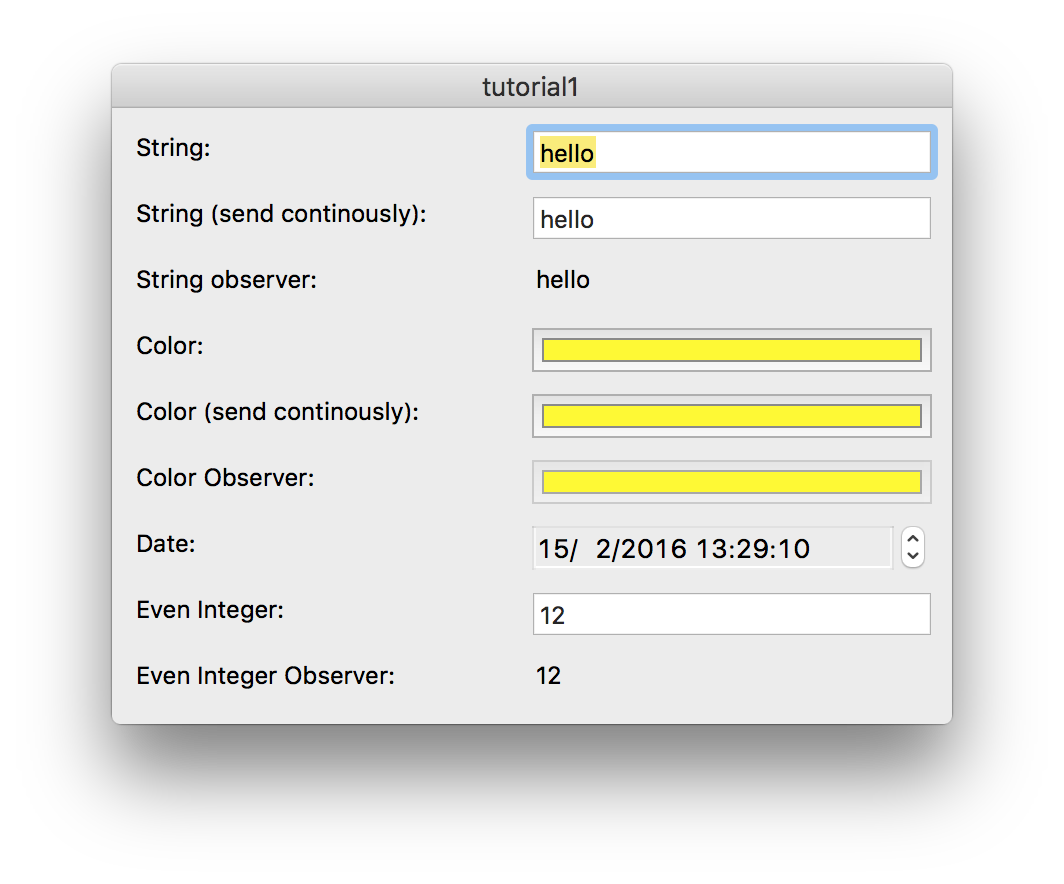
\includegraphics[width=8cm]{chapitres/tutorial1.png}
  \small
\begin{ebcode}
mainxib {
  {"String:", EBTextField myTextField},
  {"String (send continously): ", EBTextField myOtherTextField},
  {"String observer:", EBTextObserverField myObserverTextField},
  {"Color:", EBColorWell mColorWell},
  {"Color (send continously):", EBColorWell mContinousColorWell},
  {"Color Observer:", EBColorObserverWell mObserverColorWell},
  {"Date:", EBDatePicker mDatePicker},
  {"Even Integer:", EBIntField mIntegerTextField},
  {"Even Integer Observer:", EBIntObserverField mIntegerObserverTextField}
}
\end{ebcode}
  \caption{Interface graphique du premier tutorial et sa description}
  \labelFigure{interfaceGraphiquePremierTutorial}
  \ligne
\end{figure}

Après compilation Xcode, le projet est prêt à être exécuté ; le lancer fait apparaître la fenêtre illustrée par la \refFigurePage{}{interfaceGraphiquePremierTutorial}.

Les sections qui suivent sont consacrées à la description du texte source \emph{Easy Bindings}, en commençant par la clause \eb!mainxib!, suivie de la clause \eb!prefs!.







\subsectionLabel{Clause \texttt{xcodeproject}}{clauseProject}\index{xcodeproject}

La clause \eb!xcodeproject! permet d'ordonner la génération d'un projet Xcode. Le seul paramètre à fournir est la chaîne permettant de définir le « \emph{Bundle Identifier} » de l'application :
\begin{ebcode}
xcodeproject "fr.irccyn.molinaro" ;
\end{ebcode}

Le « \emph{Bundle Identifier} » de l'application est construit à partir de la chaîne fournie, en ajoutant un point suivi du nom du fichier source \emph{Easy Binding} sans son extension : pour le fichier \texttt{tutorial1.eb}, le « \emph{Bundle Identifier} » est \texttt{fr.irccyn.molinaro.tutorial1}.




\subsectionLabel{Clause \texttt{mainxib}}{clauseMainXIB}\index{mainxib}

La clause \eb!mainxib! permet de décrire une fenêtre liées aux \emph{préférences} de l'application. La présentation est systématique (\refFigurePage{}{interfaceGraphiquePremierTutorial}), deux colonnes, celle de gauche étant un commentaire, celle de droite contenant l'item graphique (bouton, champ texte, …). Ceci est uniquement destiné à réaliser rapidement des petits exemples illustratifs.

Le code est une description ligne par ligne de la composition de la fenêtre, en commençant par le haut ; Chaque ligne a la forme suivante : 
\begin{ebcode}
  {"commentaire", TypeOutlet nomOutlet}
\end{ebcode}

\eb!"commentaire"! est le texte qui est affiché dans la colonne de gauche ; \eb!TypeOutlet! et \eb!nomOutlet! sont évidemment le type et le nom de l'outlet. À noter que les types définis par Cocoa (\texttt{NSTextField}, \texttt{NSColorWell}, …) ne sont pas utilisés, au profit de types propres à \emph{Easy Bindings} : \eb!EBTextField!,  \eb!EBTextObserverField!, \eb!EBObserverWell!, \eb!EBColorObserverWell!, … La raison en est la suivante : les bindings d'\emph{Easy Bindings} nécessitent des propriétés complémentaires et un typage fort qui ne ne peuvent pas être exprimés directement avec les classes définies dans Cocoa ; les classes définies dans \emph{Easy Bindings} en héritent et implémentent les bindings.

{\bf Attention : } La vérification de la cohérence \eb!TypeOutlet! et \eb!nomOutlet! avec leur utilisation dans la clause \eb!prefs! n'est pas effectuée : une erreur n'est pas décelée lors de la compilation \emph{Easy Bindings}, et a des conséquences imprévisibles dans le projet Xcode : erreur de compilation, d'exécution, …










\subsectionLabel{Clause \texttt{prefs}}{clausePrefs}\index{prefs}

Une clause \eb!prefs! décrit modèles et bindings. Le seul couplage entre cette description et la description graphique (dans une classe \eb!mainxib! ou à la main) est constitué par les outlets et leur type. Sa compilation engendre un fichier \texttt{Preferences.swift} qui définit la classe \texttt{Preferences}.

%Un projet accepte zéro, une ou plusieurs clauses \eb!prefs! ; écrire :
%\begin{ebcode}
%prefs {
%  # définitions A
%}
%prefs {
%  # définitions B
%}
%prefs {
%  # définitions C
%}
%\end{ebcode}
%
%est équivalent à :
%\begin{ebcode}
%prefs {
%  # définitions A
%  # définitions B
%  # définitions C
%}
%\end{ebcode}

\subsubsection{Déclaration des propriétés}

Observons la première ligne de la clause \eb!prefs! (\refSubsectionPage{textSourceTutorialUn}) :
\begin{ebcode}
  property String myString default "hello" ;
\end{ebcode}

Elle déclare le modèle \eb!myString!, de type \eb!String!, dont la valeur initiale est \eb!"hello"!. Dans le code engendré, \texttt{myString} est une propriété de la classe \texttt{Preferences}. Son type est \texttt{EBStoredProperty\_String}. Cette classe prend complètement en charge l'écriture et la lecture de la valeur dans les préférences de l'application (la clef associée est \texttt{Preferences:myString}).

La valeur initiale n'est utilisée que lors du premier lancement de l'application, ou lorsqu'une propriété est ajoutée, c'est-à-dire quand la clé \texttt{Preferences:myString} n'existe pas dans les préférences de l'application.

Il en est de même pour les autres propriétés :
\begin{ebcode}
  property NSColor mColor default yellowColor ;
  ...
  property NSDate mDate default date ;
  ...
  property validates Int mIntegerValue default 12 ;
\end{ebcode}

La dernière déclaration fait apparaître le mot réservé \eb!validates! qui ordonne la validation des données saisie via l'interface ; ce point est examiné à la \refSubsubsectionTitlePage{validationSaisie}.


\subsubsection{Déclaration des outlets de leurs bindings}



\subsubsectionLabel{Validation de la saisie}{validationSaisie}


